\documentclass[a4paper,12pt]{article}

\usepackage[utf8]{inputenc}
\usepackage[german]{babel}
\usepackage{hyperref}
\usepackage[margin=3cm]{geometry}
\usepackage{graphicx}
\usepackage{graphicx}
%\usepackage{ucs}
\usepackage{minted}
\usepackage{color}

\definecolor{mygreen}{rgb}{0,0.6,0}
\definecolor{mygray}{rgb}{0.5,0.5,0.5}
\definecolor{mymauve}{rgb}{0.58,0,0.82}

\title{2D-Zeichnen im Browser}
\author{Johannes Reuter}
\date{\today}

\pdfinfo{%
  /Title    (2D-Zeichnen im Browser)
  /Author   (Johannes Reuter)
  /Creator  (Johannes Reuter)
  /Producer (Johannes Reuter)
}

\begin{document}
\maketitle
\tableofcontents
\section{Motivation}
2D-Computer-Spiele haben eine lange Tradition. Von alten Gameboy-Spielen bis hin zu modernen, grafik-gewaltigen Spielen auf modernen Spielekonsolen oder iPhone-Spiele gibt es tausende verschiedene Titel, die alle nur denkbaren Spielprinzipien, Zielgruppen und Themengebiete abdecken. Seit dem Einzug des Internets in den Massenmarkt gehören dazu auch Spiele im Browser.
Diese benötigen keine Installation, sind immer auf dem neuesten Stand und daher sowohl bei Entwicklern als auch bei Kunden beliebt. Lange Zeit wurden diese Spiele fast ausnahmslos in Flash umgesetzt, was einige Probleme mit sich brachte. Zum einen muss ein Flash-Player auf dem Endgerät installiert sein; außerdem ist der Flash-Player eine proprietäre Software und daher der vollkommenen Kontrolle der Rechte-Inhaber unterworfen. Heute gibt es verschiedene offene, standardisierte Technologien, die es ermöglichen, 2D-Browserspiele ohne Einsatz kommerzieller Software zu entwickeln und anderen zur Verfügung zu stellen. Dieses Dokument gibt einen Überblick über den Stand der momentan verfügbaren Technologien und untersucht anhand Indikatoren wie Performance, Community, Browser-Unterstützung und Framework-Verfügbarkeit, welche Technologien sich heute besonders eignen, 2D-Spiele im Browser zu entwickeln.
\section{Anforderungen}
In dieser Ausarbeitung werdend die Technologien HTML5-Canvas, WebGL, DOM-Sprites und SVG untersucht. Dabei werden der Aufbau und die Arbeitsweise vorgestellt und anschließend folgende Eigenschaften bewertet.
\paragraph{Community}
Gibt es bekannte Projekte, die die Technologie einsetzen? Hat sich ein Ökosystem aus Blogs, Foren und Hobby-Entwicklern gebildet, die dabei helfen, Fehler und Probleme zu entdecken und zu beseitigen? Gibt es Firmen oder Komitees, die die Weiterentwicklung vorantreiben oder ermutigen? Eine Technologie kann nur überleben, wenn sich eine solche Community entwickelt, die das Projekt ständig weiterentwickelt und an neue Anforderungen anpasst.
\paragraph{Frameworks}
Gibt es Frameworks, die eine abstrakte, einfach zu verwendende API bereitstellen? Sind diese praxistauglich und umfangreich, gibt es Plugins und Erweiterungen? Nicht nur sind solche Projekte eine guter Indikator dafür, dass sich Menschen mit der Technologie beschäftigen und sie auf Tauglichkeit überprüfen, ohne solche Hilfsmittel wird es in der Praxis oft sehr schwierig, echte, große Anwendungen umzusetzen.
\paragraph{Unterstützung}
Ist es überhaupt möglich, die Technologie in der Praxis einzusetzen, oder befindet sich diese noch im Beta-Stadium? Da die Zielgruppe bei Browser-Spielen sehr groß ist und eine Vielzahl von verschiedenen Plattformen und Browsern verwendet wird, ist eine große Verbreitung und eine stabile Laufzeitumgebung auf möglichst vielen Geräten ein großes Plus wenn nicht sogar essentiell.
\paragraph{Performance}
Die Technologie selbst mag den anderen Anforderungen genügen, aber ist die Leistung ausreichend für einen flüssigen Spielablauf? Gerade im Browser, wo die Performance generell etwas schlechter wie z.B. bei Desktop-Anwendungen ist, muss auf diesen Punkt besonders viel Rücksicht genommen werden. Auch hier muss die Vielzahl der Endgeräte und Plattformen mit zum Teil sehr deutlich unterschiedlichen Rechenleistungen beachtet werden.
\section{Performance-Messung}
Zur Performance-Messung der verschiedenen Technologien habe ich eine einfache Beispiel-Anwendung in Javascript geschrieben: Objekte bewegen sich mit einem konstanten Vektor in einer begrenzten zweidimensionalen Welt und prallen an Wänden und Decken ab. Die Spiele-Physik ist ein eigenständiges Javascript-Modul, das auf eine belibiege Implementierung der Oberfläche zurückgreifen kann: Canvas, WebGL, SVG oder DOM. Das Oberflächen-Modul wurde für jede Technik neu implementiert. Um einen vergleichenden Wert zu ermitteln, wird die Anzahl der Objekte in der Spiele-Welt so lange erhöht, bis 30 FPS erreicht sind. Dieser Benchmark-Test wird dann in verschiedenen Browsern wiederholt, um Unterschiede zu ermitteln.
\inputminted{javascript}{assets/benchmark1.js}
\inputminted{javascript}{assets/benchmark2.js}
\section{HTML5-Canvas}
\subsection{Technologie}
\paragraph{} Das Canvas-Element (englisch für Leinwand) und die entsprechende Javascript-API ist vom W3C spezifiziert und wird von allen großen Browser-Herstellern implementiert. Dadurch ist gesichert, dass ein Browser-Spiel, das das Canvas-Element zur Darstellung nutzt, in auch vielfältigen  Umgebungen korrekt funktioniert. Auch WebGL gehört zum Canvas-Standard, da das Canvas-Element verschiedene Kontexte unterstützt; dieses Kapitel behandelt jedoch ausschließlich den \glqq 2d\grqq-Kontext, der \glqq webgl\grqq-Kontext wird im Kapitel \emph{WebGL} behandelt.
\paragraph{API} Die Canvas-API zeichnet sich besonders durch Schlichtheit und eine niedrige Lernkurve aus. Dabei ist der Zeichen-Kontext als Zustandsautomat implementiert, d.h. es werden nicht alle Informationen zum Zeichnen einer Linie in einem Methoden-Aufruf mitgegeben, sondern in mehreren. Erst wird der Zeichen-Stil konfiguriert, dann wird der Pfad definiert und dann die Linie gezeichnet.
\begin{minted}{javascript}
context.strokeStyle = '#fa00ff'; //definiere Farbe
context.lineWidth = 5; //definiere Stift-Breite
context.lineCap = 'round'; //definiere Linien-Abschluss
context.beginPath(); //definiere pfad
context.moveTo(0,0); //...
context.lineTo(100,100); //...
context.stroke(); //zeichne linie mit obigen einstellungen
\end{minted}
Da in der Praxis meist mehrere Zeichenoperationen mit der selben Konfiguration durchgeführt werden, hat dies den Vorteil dass so Rechenleistung gespart werden kann und der Quellcode einfacher bleibt.
\paragraph{Umfang} Mit dem Canvas-Element lassen sich unter anderem folgende Dinge zeichnen:
TODO: quote wikipedia here
\begin{itemize}
	\item Linien (gestrichelt, durchgezogen, ...)
	\item (gefüllte) Rechtecke
	\item Kreisbögen
	\item (gefüllte) Ellipsen
	\item Bezierkurven
	\item Gradienten
	\item Pixel-Grafiken (alles, was mit dem Image-Objekt geladen werden kann)
	\item Text
	\item Transparenz
\end{itemize}
Damit ist es perfekt geeignet, um auch aufwendige 2D-Spiele darzustellen, die meistens aus Serien von Pixelgrafiken bestehen, die in schneller Folge eingeblendet werden (sogenannte \emph{Sprites}).
\subsection{Unterstützung}
\begin{figure}[h!]
	\begin{center}
		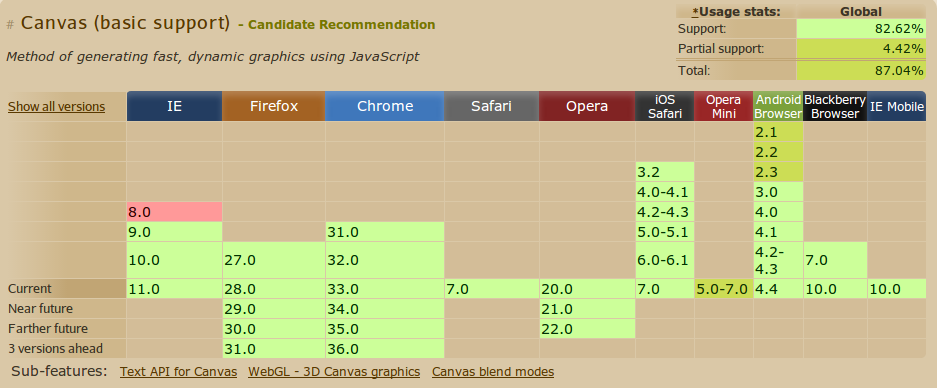
\includegraphics[width=\textwidth]{assets/canvas_support.png} 
	\end{center}
	\caption{Canvas Unterstützung}
	\label{canvas_support}
\end{figure}
Der 2D-Kontext wird von allen modernen Browsern unterstützt, Opera Mini bildet hier die einzige Ausnahme; sogar mobile Browser bieten die API durchgehend an. Sogar Internet-Explorer, der dafür bekannt ist, bei der Untersütztung von Standarts aus dem Rahmen zu fallen, bietet Canvas ab der Version 9.0 an. Natürlich gibt es viele Internet-Nutzer, die auch sehr alte Versionen von Browsern benutzen, allerdings sind diese für die Zielgruppe der online Spielenden Bevölkerung nicht besonders relevant; die meisten dieser alten Browser werden in Firmen mit veralteter IT-Technik benutzt, wo das Spielen am Computer sowieso verboten ist.
TODO: bild vom support einbinden.
\subsection{Frameworks}
Canvas ist die mit Abstand am weitesten verbreitete der hier vorgestellten Technologien. Dies ist wohl vor allem der niedrigen Lernkurve und dem schnellen Einstieg mit frühen Erfolgen zu danken. Daher ist die Community sehr aktiv und hat unzählige Tools, Bibliotheken und Frameworks entwickelt. Die wichtigsten dieser Tools werden hier in Kürze vorgestellt:
\subsubsection{KineticJS}
KineticJS ist ein auf HTML5 Canvas spezialisiertes, quelloffenes Framework, d.h. es bietet keinen Technologie-Fallback an. Es abstrahiert die Canvas-API und bietet eine Objekt-Orientier
te API an, in der \emph{Shapes} definiert werden, die zu Gruppen zusammengefasst werden und dann verschiedenen \emph{Layers} zugeordnet werden. Die Layer zusammen bilden den Szene-Graph
en, der alle dargestellten Objekte beinhaltet. Die einzelnen Objekte der Szene können jetzt unabhängig animiert und transformiert werden. Dabei ist nicht nur Rotation und Translation mö
glich, sondern z.b. auch Farb-Transformation u.Ä. Dazu kommt noch eine ereignis-basierte Architektur, mit der Animationen synchronisiert werden können.
\paragraph{Beispiel}
Anbei ein kleines Beispiel, wie der KintectJS-Code aussieht. In diesem Beispiel wird eine neue Szene (auch Stage genannt) angelegt und ein rotes Dreieck an einer zufälligen Position angezeigt.
\inputminted{javascript}{assets/kineticjs_example.js}
\paragraph{Verwendung} KineticJS wird bereits in vielen verschiedenen aktiven Projekten eingesetzt, auf http://kineticjs.com/ gibt es eine ganze Auswahl von verschiedenen Browser-Spiele
n, die mit diesem Framework entwickelt wurden. Im Entwickler-Forum Stackoverflow gibt es hunderte Fragen zum Thema und über Google lassen sich Dutzende Tutorials finden, wie kleine Spie
le mit KineticJS entwickelt werden können.
\subsubsection{EaselJS}
EaselJS ist ein Framework, dessen API an Flash angelehnt ist. So fällt der Übergang leichter. Darüber hinaus existieren verschiedene Tools, die alle auf (ehemalige) Flash-Entwickler abzielen. Zum Beispiel gibt es EaselFL, ein Flash-Fallback für alte Browser, die Canvas nicht unterstützen, oder Zoe, ein Exporter für SWF-Animationen in EaselJS-Spritesheets.
\paragraph{TweenJS/SoundJS/PreloadJS} EaselJS kümmert sich nur um die reine Arbeit mit HTML5 Canvas, Funktionen wie Animationen und Transformationen oder Sounds sind in eigenen Modulen gekapselt:
\begin{itemize}
	\item \emph{TweenJS} für Animationen und Transformationen
	\item \emph{SoundJS} für Arbeiten mit Sounds
	\item \emph{PreloadJS} für das Managen und Laden von Bildern und Spiele-Inhalten
\end{itemize}
Damit ist die EaselJS-Suite nicht nur ein Framework für das Arbeiten mit Canvas, sondern bietet Werkzeuge, um ganze Browser-Spiele oder andere Anwendungen zu entwickeln.
\subsection{Beispiel}
Wie bereits erwähnt, ist die API von Canvas sehr schlicht und einfach zu erlernen. Dabei spielt sich alles im sogenannten Context-Objekt ab. Auf diesem können Methoden aufgerufen werden, um Bilder oder Linien auf  die Arbeitsfläche zu zeichnen. Um Animationen oder ähnliches zu realisieren, empfiehlt es sich, die Methode requestAnimation-Frame zu verwenden.
\paragraph{requestAnimationFrame} Diese Methode bekommt als Parameter eine Funktion übergeben, die nach gewisser Zeit vom Browser aufgerufen wird. Üblicherweiße ruft diese Funktion rekursiv wieder requestAnimationFrame mit sich selbst als Parameter auf. Der Browser fungiert hier als Balancer und sorgt dafür, dass die Methode nicht öfter aufgerufen wird als nötig. So wird zum Beispiel die Framezahl pro Sekunde beschränkt und keine weiteren Aufrufe angefordert, wenn das Browser-Fenster nicht im Vordergrund ist. Um die Ablaufgeschwindigkeit des Spiels vom Verhalten der requestAnimationFrame-Methode zu entkoppeln, muss bei jedem Aufruf ermittelt werden, wie viel Zeit seit dem letzten Aufruf vergangen ist und zum Beispiel Bewegungs-Vektoren entsprechend angepasst werden.
\inputminted{javascript}{assets/vanillacanvas_example.js}
\subsection{Performance}
\section{WebGL}
\subsection{Technologie}
\subsection{Frameworks}
\subsection{Beispiel}
\subsection{Performance}
\section{DOM}
\subsection{Technologie}
\subsection{Frameworks}
\subsection{Beispiel}
\subsection{Performance}
\section{SVG}
\subsection{Technologie}
\subsection{Frameworks}
\subsection{Beispiel}
\subsection{Performance}
\section{Fazit}
\section{Ausblick}
\end{document}
